\cleardoublestylepage{common}

\section{CWA指导的SMD框架:CWA-SMD}

将CWA方法与SMD方法结合起来的最为直接的方法便为CWA指导SMD:即通过CWA演化后得到的一系列期望值作为SMD方法的截断。我们从初始的波函数进行维格纳变换得到相空间分布,
\begin{equation}
  \mathcal{W} \left[ \psi \right] (\boldsymbol{X}, \boldsymbol{P}) = \left(\frac{1}{2\pi \hbar}\right)^n \int \psi^\dagger(\boldsymbol{X}-\boldsymbol{Y}/2) \psi(\boldsymbol{X} + \boldsymbol{Y}/2) e^{i \boldsymbol{P} \cdot \boldsymbol{Y} / \hbar} \, \mathrm{d}\boldsymbol{Y} 
\end{equation}
其中$\boldsymbol{X}, \, \boldsymbol{P}$分别代表体系的位移自由度和平移自由度,并以此相空间分布为基础得到的任意可观察量的期望值必定是精确的。同时,将其进行离散化处理,对初始波函数$\psi_0(\boldsymbol{X})$及其对应相空间分布$ \Gamma_0(\boldsymbol{X}, \boldsymbol{P}) = \mathcal{W}\left[ \psi_0(\boldsymbol{X}) \right] $, 做近似
\begin{equation}
  \Gamma_0 (\boldsymbol{X}, \boldsymbol{P}) \sim \sum_{k} \Gamma_{k}'(\boldsymbol{X}, \boldsymbol{P}) = \sum_{ij} c_{ij} \delta(\boldsymbol{X} - \prescript{0}{}{\boldsymbol{q}_k}) \delta(\boldsymbol{P} - \prescript{0}{}{\boldsymbol{p}_k})
\end{equation}
其中$\left\{ \prescript{0}{}{\boldsymbol{q}_k}, \prescript{0}{}{\boldsymbol{p}_k} \right\} $ 为相空间某区域均匀分布的格点,以及
\begin{equation}
  c_{k} = \int \Gamma_0(\boldsymbol{X}, \boldsymbol{P}) \delta(\boldsymbol{X} - \prescript{0}{}{\boldsymbol{q}_k}) \delta(\boldsymbol{P} - \prescript{0}{}{\boldsymbol{p}_k}) \, \mathrm{d}\boldsymbol{X}\mathrm{d}\boldsymbol{P}
\end{equation}
演化利用泊松括号来实现,
\begin{equation}
\frac{\mathrm{d}}{\mathrm{d}t} \Gamma'_{k}(\boldsymbol{X}, \boldsymbol{P})
\begin{cases}
	\frac{\mathrm{d} c_{k}}{\mathrm{d} t} = 0 , \\
	\frac{\mathrm{d} \boldsymbol{q}_k}{\mathrm{d} t} = \frac{\boldsymbol{p}_k}{m} , \\
	\frac{\mathrm{d} \boldsymbol{p}_k}{\mathrm{d} t} = - \frac{\partial V(\boldsymbol{X})}{\partial \boldsymbol{X}}\bigg|_{\boldsymbol{X} = \boldsymbol{q_k}}
\end{cases}
\end{equation}
该部分即为CWA的演化方法,同时不受SMD方法的干涉。对于SMD部分,准备$\boldsymbol{X}$与$\boldsymbol{P}$的幂函数$\{\Xi_i(\boldsymbol{X},\boldsymbol{P})\}$或其他存在迭代形式的函数形式作为可观察量组,构建演化方程
\begin{equation}
\frac{\mathrm{d}}{\mathrm{d} t} \langle \Xi_i(\boldsymbol{X},\boldsymbol{P}) \rangle = \langle \{\{\Xi_i(\boldsymbol{X},\boldsymbol{P}), H\}\} \rangle
\end{equation}
其中 $\{\{ *, * \}\}$为磨雅括号,定义为
 \begin{equation}
	 \{\{f, g\}\}=\frac{2}{\hbar} f \sin \left[\frac{\hbar}{2}\left(\sum_{i} \overleftarrow{\partial}_{q_{i}} \overrightarrow{\partial}_{p_{i}}-\overleftarrow{\partial}_{p_{i}} \overrightarrow{\partial}_{q_{i}}\right)\right] g
\end{equation}
由于哈密顿量也同时为$\boldsymbol{X}$与$\boldsymbol{P}$的幂函数,$\{\{P_i(\boldsymbol{X},\boldsymbol{P}), H\}\}$亦为一系列幂函数的线性组合,
\begin{equation}
\{\{\Xi_i(\boldsymbol{X},\boldsymbol{P}), H\}\} = \sum_k c_k \Xi_k(\boldsymbol{X},\boldsymbol{P})
\end{equation}
。在演化过程中,若$P_k(\boldsymbol{X},\boldsymbol{P})$被涵盖于$\{P_i(\boldsymbol{X},\boldsymbol{P})\}$,那么直接引用该期望值做演化,否则使用CWA的分布函数做近似,
\begin{equation}
\langle \Xi_k(\boldsymbol{X},\boldsymbol{P}) \rangle = \sum_{ij} c_{ij} \Xi_k(\boldsymbol{q}_i,\boldsymbol{p}_j)
\end{equation}
阶数对应了$\{P_i(\boldsymbol{X},\boldsymbol{P})\}$所包含的最高次。 

\begin{figure}
\centering
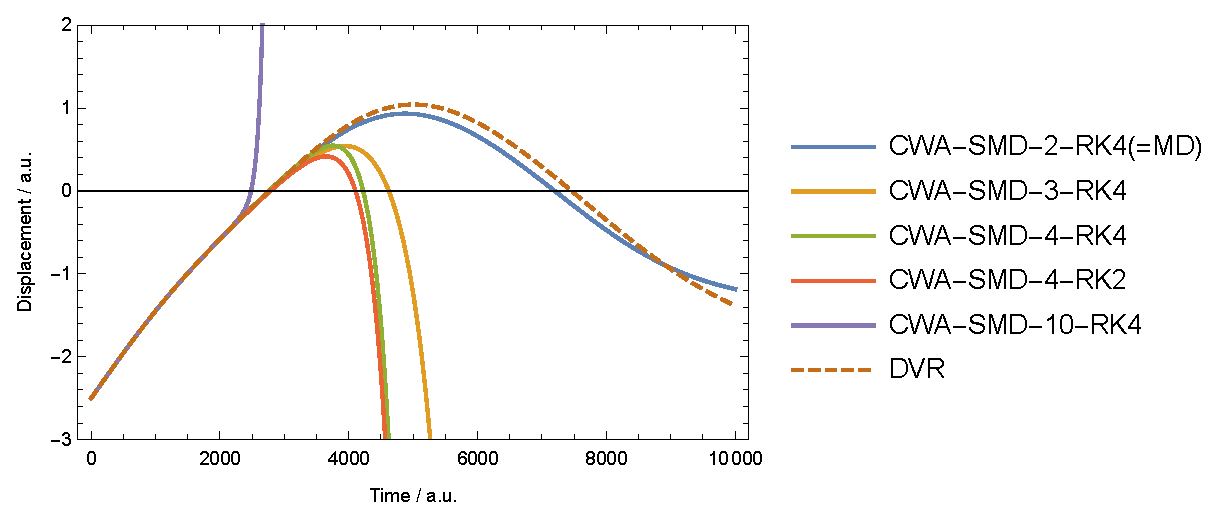
\includegraphics[width=0.8\textwidth]{cwa_smd.eps}
\caption{双势阱模型中CWA-SMD方法的演化结果与DVR、CWA的对照}
\label{cwa-smd-double-well}
\end{figure}

在实际演化过程中,对于CWA相空间分布的格点坐标演化以及SMD追踪的可观察量的期望值的演化都使用相同的数值求解常微分方程的框架,在本次论文中主要使用Runge-Kutta系列。我们主要考察双势阱模型,其势能函数及初始波函数的定义为
\begin{equation}
\begin{cases}
V(x) = 0.000024 x^4 - 0.0003 x^2 \\
\psi(x) = e^{-(x+2)^2} e^{2ix} \\
m = 1836
\end{cases}
\end{equation}

其结果如图 \ref{cwa-smd-double-well}所示。其中,CWA-SMD后的数字代表了追踪的可观察量的最高阶数,而更高阶的可观察量的期望值由CWA近似提供。作为示例,CWA-SMD-5只追踪1至5阶的可观察量的期望值(如 $x$, $p^2$, $x^2 p^3$等)。每个维度选取[-10 a.u., 10 a.u.]区间内的50个格点,即演化过程中总共有2500个格点,并使用1.0 a.u.作为模拟的时间元。可以明显看出,高于2阶的CWA-SMD方法都在$t=3000 \,\mathrm{a.u.}$附近与精确解(DVR)发生偏离,同时误差不断累积直至发生绝对性的偏差。而CWA-SMD-2的结果与CWA方法一致的原因是不高于2阶的可观察量($x, p, xp, x^2, p^2$)在磨雅括号下给出的演化方程与经典力学中的泊松方程一致(因为不存在三阶及以上的偏导,对应的项不贡献)。而CWA的演化过程只考虑经典力学部分,因此CWA方法与CWA-SMD-2方法事实上会给出相同的结果。同时我们可以看出,不同的Runge-Kutta方法(RK2,RK4)对体系演化的影响不大,说明数值求解常微分方程框架并非为CWA-SMD未能收敛的决定性因素。

\begin{figure}
\centering
\subfigure[绝对误差]{
	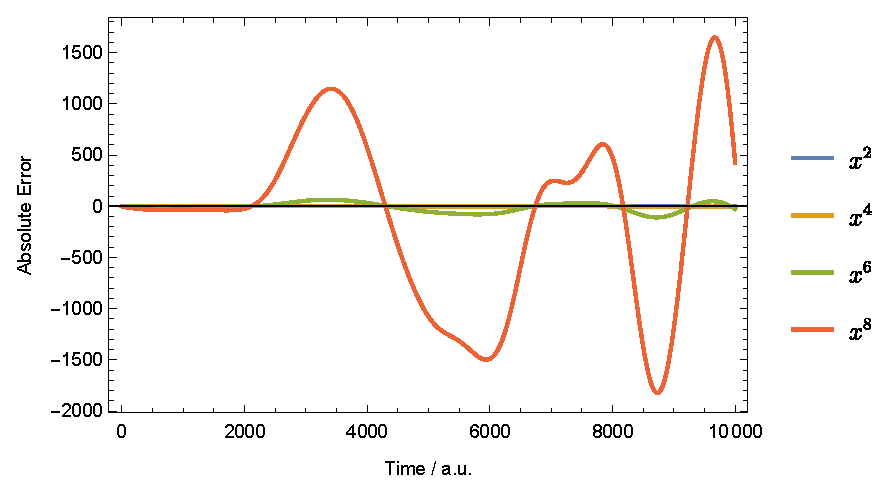
\includegraphics[width=0.48\textwidth]{cwa_exp_absolute_error.eps}	
}
\subfigure[相对误差]{
	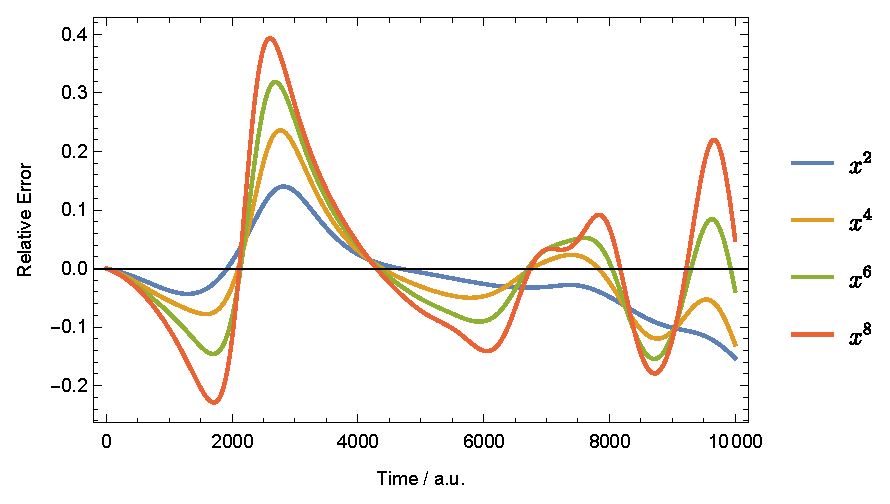
\includegraphics[width=0.48\textwidth]{cwa_exp_relative_error.eps}
  \label{cwa-smd-relative-error}
}
\caption{双势阱模型中CWA方法给出的一些典型的可观察量的期望值与DVR方法的差异}
\label{exp-error}
\end{figure}
为研究CWA-SMD方法产生的误差的来源,我们考察了在该模型下DVR方法与CWA方法在高阶可观察量下的期望值的差异,如图 \ref{exp-error}所示。其非常显著地揭示了CWA方法在高阶可观察量的期望值与DVR精确解提供的期望值之间的误差,且其随着可观察量阶数的提升而有显著的增加。从图 \ref{cwa-smd-relative-error} 可以看出体系在$t=2000 \,\mathrm{a.u.}$附近便开始有显著的量子效应,而在$t=3000 \,\mathrm{a.u.}$时更为显著。而这些高阶可观察量的期望值的误差会在体系演化过程中逐渐渗透于低阶可观察量的期望值,最终在位移的期望值中体现出来,发生偏离,而这从图 \ref{cwa-smd-double-well}高阶CWA-SMD方法发生偏离的时间点在$t=2000 \,\mathrm{a.u.}$附近,低阶CWA-SMD方法在$t=3500 \,\mathrm{a.u.}$附近发生偏离的现象基本吻合。

\begin{figure}
\centering
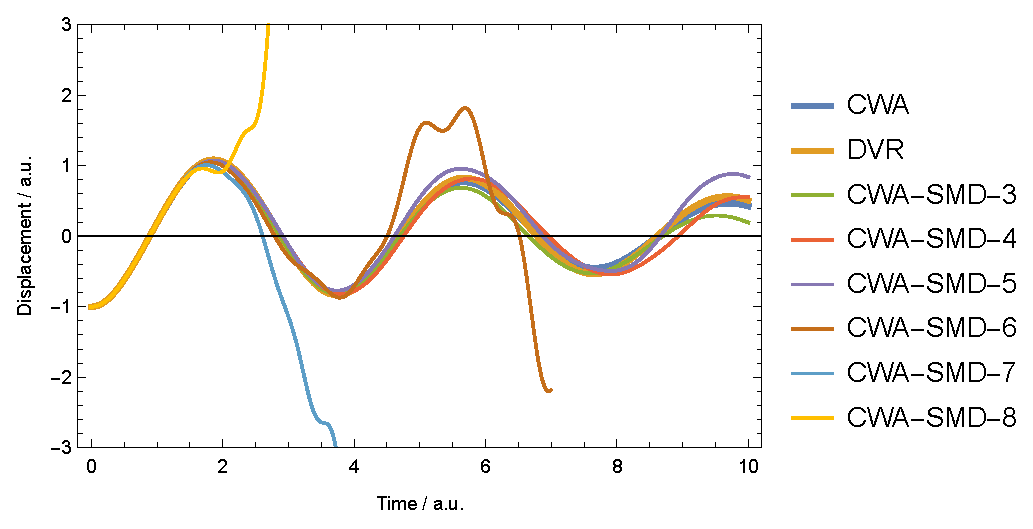
\includegraphics[width=0.8\textwidth]{anharmonic_cwa_smd.eps}
\caption{非谐性振子模型中CWA-SMD方法的演化结果与DVR、CWA的对照}
\label{cwa-smd-anharmonic}
\end{figure}

\begin{figure}
\centering
\subfigure[绝对误差]{
  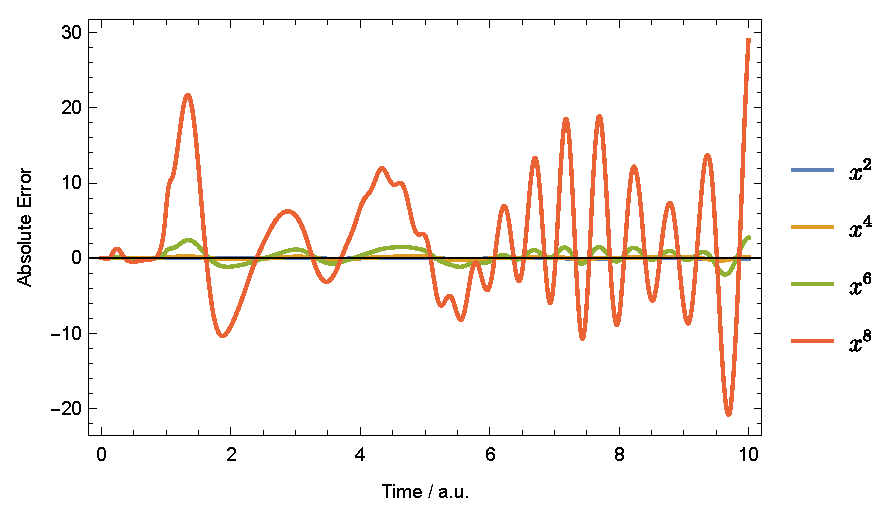
\includegraphics[width=0.48\textwidth]{cwa_exp_absolute_error_anharmonic.eps} 
}
\subfigure[相对误差]{
  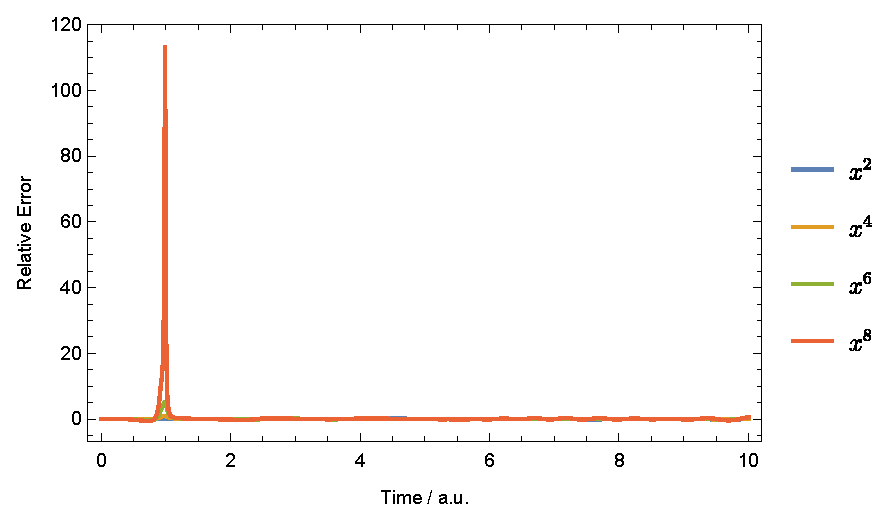
\includegraphics[width=0.48\textwidth]{cwa_exp_relative_error_anharmonic.eps}
    \label{cwa-smd-relative-error-anharmonic}
}
\caption{非谐性振子模型中CWA方法给出的一些典型的可观察量的期望值与DVR方法的差异}
\label{exp-error-anharmonic}
\end{figure}

我们同时考察了非谐性振子模型,其势能函数及初始波函数的定义为\cite{liu2007real}
\begin{equation}
\begin{cases}
V(x) = x^2 - 0.1 x^3 + 0.1 x^4 \\
\psi(x) = e^{-\frac{(x+1)^2}{2}} \\
m = 1
\end{cases}
\end{equation}
其结果如图 \ref{cwa-smd-anharmonic}所示,CWA方法与DVR方法在高阶可观察量的差异如图 \ref{exp-error-anharmonic}所示。该模型相对于双势阱模型有着较好的结果,但对于高阶的CWA-SMD方法的收敛性仍不尽人意。从图 \ref{cwa-smd-relative-error-anharmonic}可以看出在$t= 1 \, \mathrm{a.u.}$有非常显著的量子效应,而这也是高阶CWA-SMD方法(CWA-SMD-7与CWA-SMD-8)发生崩坏的时间点($t= 5 \, \mathrm{a.u.}$)基本一致。而较低阶的CWA-SMD方法能最终不发生数值崩坏则可能是由于后期的震荡,使误差不至于积累过多,从而能够运行至最后。然而由于高阶量的误差的积累,相比CWA与精确解有更大的偏离。

因此,综合而言CWA-SMD不足以改善CWA的演化轨迹,而CWA在高阶可观察量的期望值上带来的误差会使CWA-SMD相对于DVR的偏差更大。

\newpage
\section{SMD指导CWA的框架:CWA-SMD-OPT与SMD-CWA-OPT}
我们可以看到,由于CWA并不接受SMD的反馈,其在体系的演化过程中特别是在高阶可观察量的期望值的误差会持续不断地进入SMD的框架中并参与循环,最终导致CWA-SMD框架的位移的期望值的演化与DVR方法产生了偏差。因此我们希望通过SMD已有的数据反过来对CWA进行某种程度上的变化,使CWA能够给出更接近``正确''的相空间分布,从而得到更好的高阶可观察量的期望值,从而实现更好的SMD演化。

我们注意到,SMD一直都在追踪一定阶数范围内的可观察量的期望值,同时越接近初始时刻这些值越接近实际体系应该有的期望值——这意味着在演化过程中,SMD的期望值相对CWA给出的高阶可观察量的期望值更值得信赖。或者说,我们希望SMD与CWA是``自洽''的,即SMD与CWA在一定阶数范围内的可观察量能够提供相同的期望值。而这就意味着我们需要调整CWA的相空间分布,使调整过后的相空间分布能够提供与SMD相同的可观察量的期望值。

由于CWA本身需要较为庞大的格点数以保证对相空间分布的描述的准确度,而SMD只能追踪相对有限的可观察量(如3阶,4阶等),因此整体而言CWA的自由度远大于SMD能够提供的约束方程,因此我们无法通过解方程组的方式获得新的相空间分布。然而我们可以通过优化收敛的方式进行:我们可以通过设置一个恒正的惩罚函数,定义CWA提供的可观察量期望值与SMD追踪的可观察量的期望值之间的距离,而后利用该惩罚函数对CWA的相空间分布进行优化,从而实现我们先前提到的使CWA的可观察量期望值与SMD可观察量相一致的想法,完成``SMD指导CWA''的效果。事实上,在动力学领域已有通过设立惩罚函数优化相空间参数的先例。

而针对具体的优化方法,最常用的方式即为梯度下降法:利用额外提供的惩罚函数关于所有自由度的梯度,确定优化参数的方向,而后通过某种算法确定行进的步长而加速收敛,最终达到使惩罚函数值最低的效果。其中以BFGS法(Broyden–Fletcher–Goldfarb–Shanno algorithm)最为著名\cite{nazareth1979relationship},其利用历史的梯度数据生成近似的二阶梯度,从而更好地确定优化方向及优化步长。同时其变种BFGS-2方法被认为是最为高效的梯度下降法\cite{galassi2002gnu}。同时被学术界广泛使用的梯度下降法还有共轭梯度下降法(包括Fletcher-Reeves conjugate gradient algorithm\cite{dai1996convergence},Polak-Ribiere conjugate gradient algorithm\cite{klessig1972efficient}),以及经典的最速下降法\cite{curry1944method}。为方便地进行比较,我们使用了GSL库(GNU Scientific Library)来实现这些梯度下降的方法\cite{galassi2002gnu}。

为方便求得惩罚函数关于CWA方法中格点坐标的梯度,我们使用二次函数型。但需要注意的是,由于不同阶数的可观察量的期望值存在数量级的差别,在毫无修正的情况下会出现不同阶数的可观察量之间的偏袒,同时容易出现统一的优化收敛的标准下难以收敛的问题。因此我们需要引入放缩因子(Scaling Factor)使不同可观察量的期望值在相近的数量级下,方便进行优化。

对于CWA-SMD给出的可观察量组$\Xi_i(\boldsymbol{X},\boldsymbol{P})$, 定义放缩因子为$\{s_X,s_P\}$,使
\begin{equation}
    \mathcal{X}, \mathcal{P} \equiv \frac{\boldsymbol{X}}{s_X},\frac{\boldsymbol{P}}{s_P}
  \end{equation}
  这样的话可观察量组
  \begin{equation}
    \Xi_i(\mathcal{X},\mathcal{P}) = \Xi_i(\frac{1}{s_X},\frac{1}{s_P}) \Xi_i(\boldsymbol{X},\boldsymbol{P}) 
  \end{equation}
  定义误差函数$\Theta(\theta;\theta_0) \equiv (\theta-\theta_0)^2$,即:
  \begin{equation}
    \Theta(\{\langle \Xi_i(\mathcal{X},\mathcal{P}) \rangle \}, \{\langle \Xi_i(\mathcal{X},\mathcal{P}) \rangle \}_\mathrm{ref}) \equiv \sum_i (\langle \Xi_i(\mathcal{X},\mathcal{P}) \rangle- \langle \Xi P_i(\mathcal{X},\mathcal{P}) \rangle_\mathrm{ref})^2
  \end{equation}
其中$\mathrm{ref}$代表SMD追踪的可观察量的期望值。其关于CWA相空间分布中格点坐标的梯度为
\begin{equation}
  \nabla \Xi = \sum_i 2\left[\langle \Xi_i(\mathcal{X},\mathcal{P}) \rangle- \langle \Xi_i(\mathcal{X},\mathcal{P}) \rangle_\mathrm{ref} \right] \nabla\langle \Xi_i(\mathcal{X},\mathcal{P}) \rangle
\end{equation} 
其中$\langle \Xi_i(\mathcal{X},\mathcal{P}) \rangle_\mathrm{ref}$由于与CWA相空间分布无关故无贡献。而
\begin{equation}
  \nabla \langle \Xi_i(\mathcal{X}, \mathcal{P}) \rangle = \nabla \sum_{k} c_{k} \Xi_i (\frac{x_k}{s_X} ,\frac{p_k}{s_P}) =  \{ \frac{c_{k}}{s_X} \frac{\partial}{\partial \boldsymbol{X}} \Xi_i ( \frac{x_k}{s_X} ,\frac{p_k}{s_P}), \frac{c_{k}}{s_P} \frac{\partial}{\partial \boldsymbol{P}} \Xi_i (\frac{x_k}{s_X} ,\frac{p_k}{s_P}) \}
\end{equation} 

\subsection{SMD-CWA-OPT}
值得注意的是,此时有两种方法提供各阶可观察量的期望值:一是直接从优化完毕的CWA分布获得新的可观察量的期望值,而是从SMD一直追踪的可观察量的期望值获得。为方便起见,我们先针对CWA分布提供期望值的方法——SMD-CWA-OPT进行分析。
\begin{figure}
\centering
\subfigure[2阶]{
  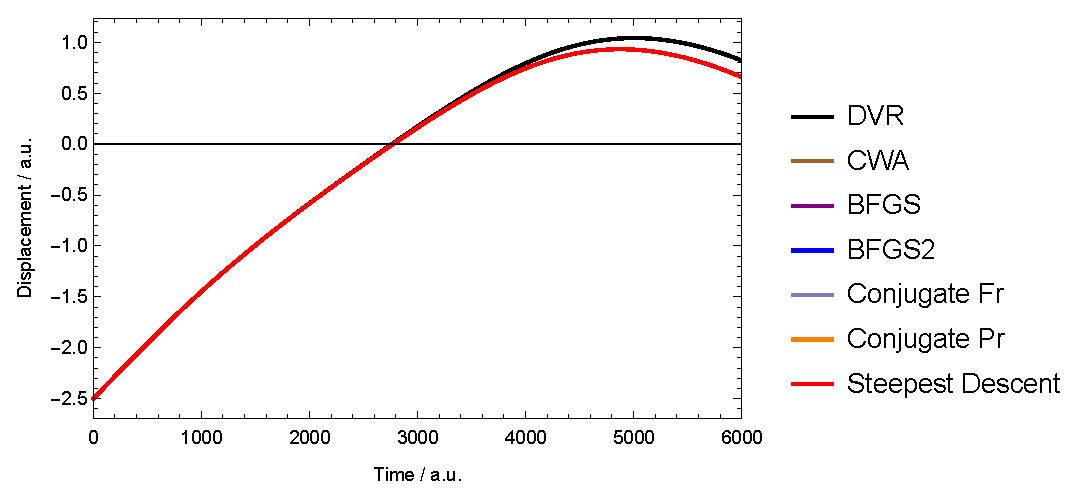
\includegraphics[width=0.48\textwidth]{SMD_CWA_OPT_Methods_3.eps}
  \label{smd-cwa-opt-2-method}
}
\subfigure[3阶]{
  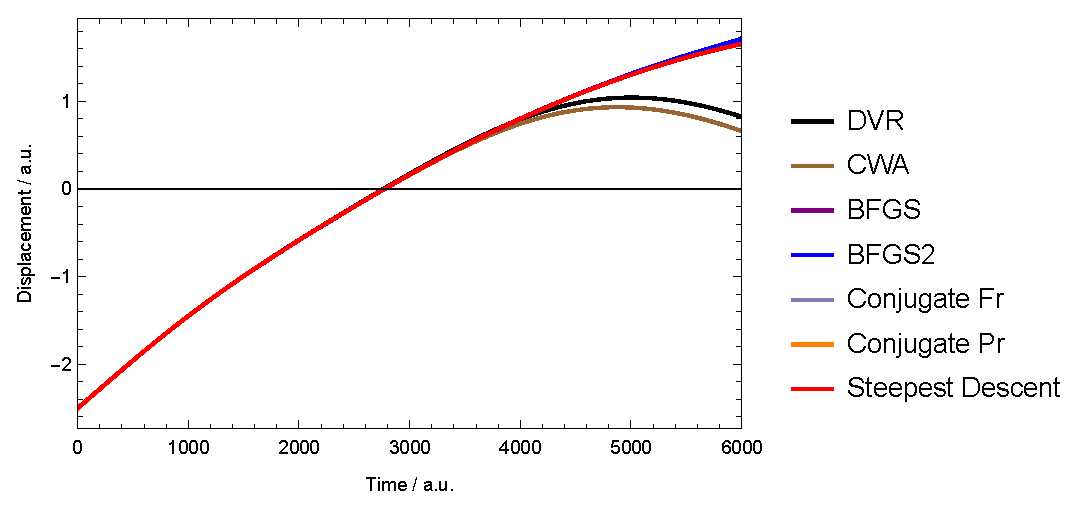
\includegraphics[width=0.48\textwidth]{SMD_CWA_OPT_Methods_4.eps}
}
\subfigure[4阶]{
  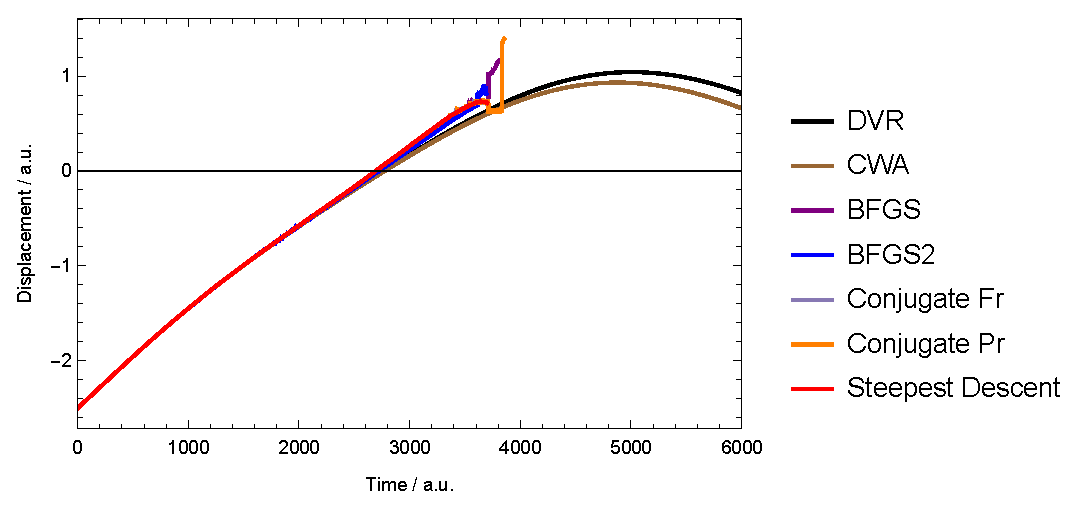
\includegraphics[width=0.48\textwidth]{SMD_CWA_OPT_Methods_5.eps}
}
\subfigure[5阶]{
  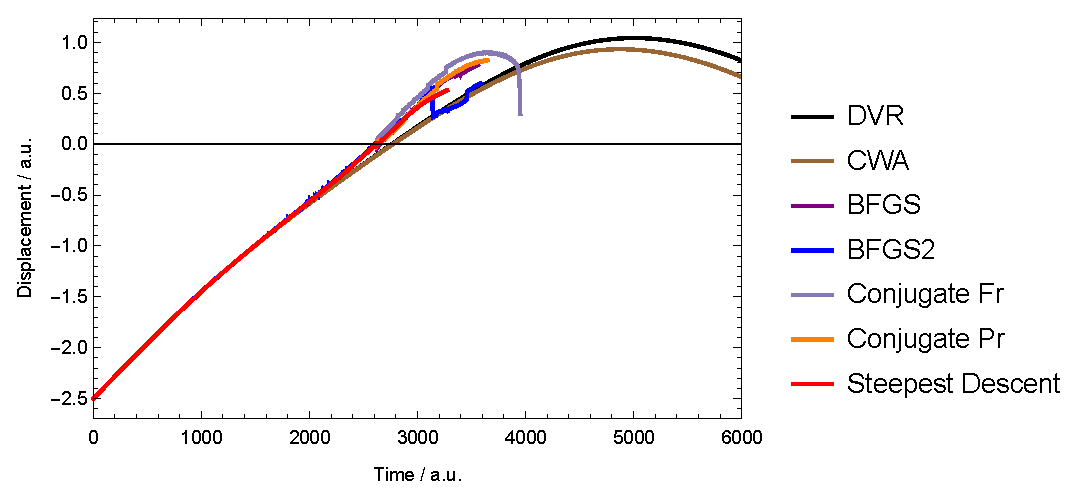
\includegraphics[width=0.48\textwidth]{SMD_CWA_OPT_Methods_6.eps}
}
\subfigure[8阶]{
  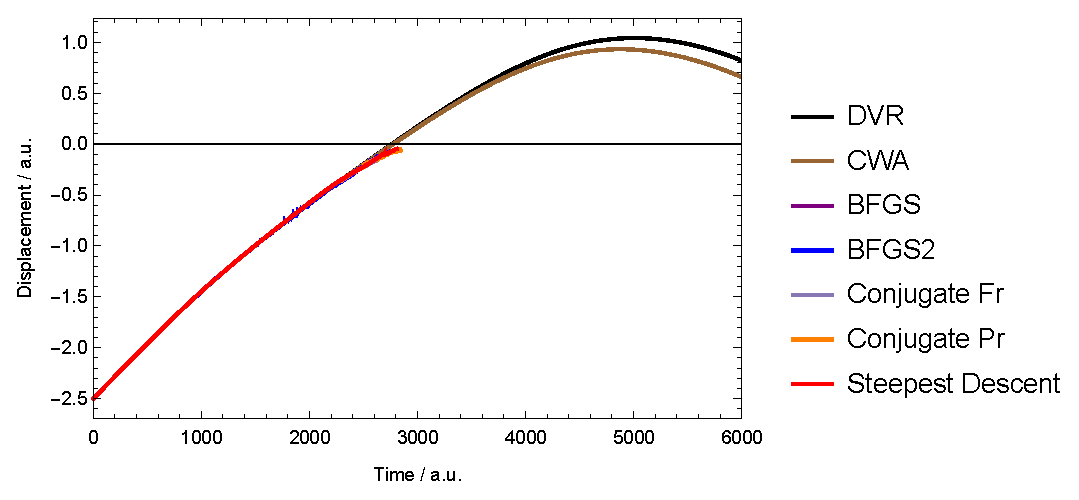
\includegraphics[width=0.48\textwidth]{SMD_CWA_OPT_Methods_8.eps}
}
\caption{不同的梯度收敛方法对SMD-CWA-OPT方法的影响}
\label{smd-cwa-opt-method}
\end{figure}

\begin{figure}
\centering
\subfigure[3阶]{
  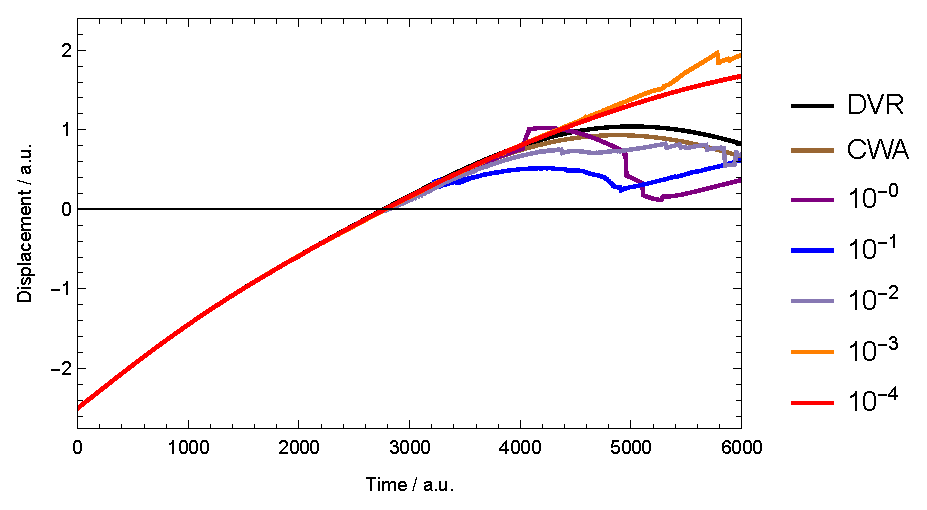
\includegraphics[width=0.48\textwidth]{SMD_CWA_OPT_init_4.eps}
}
\subfigure[4阶]{
  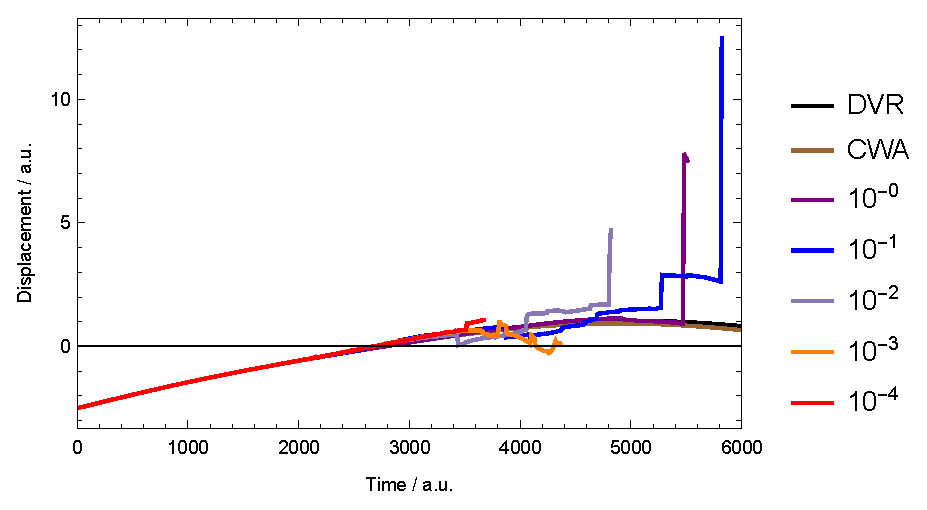
\includegraphics[width=0.48\textwidth]{SMD_CWA_OPT_init_5.eps}
}
\subfigure[5阶]{
  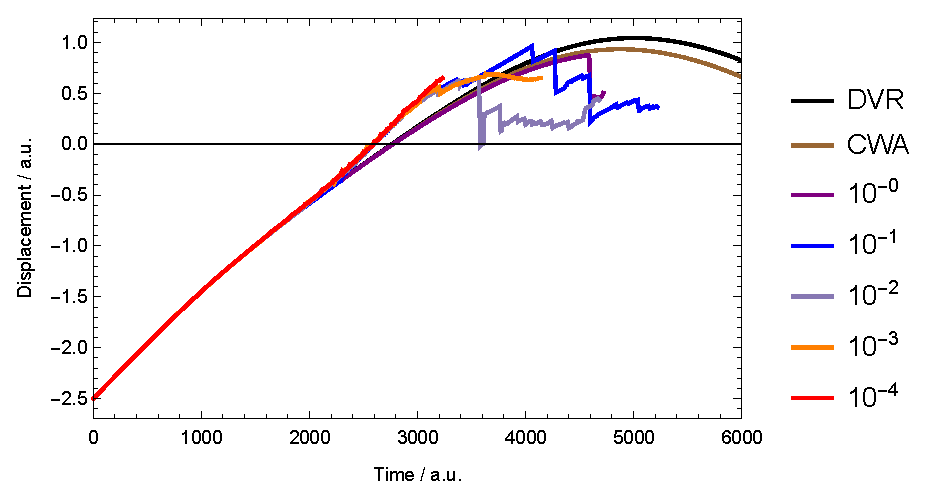
\includegraphics[width=0.48\textwidth]{SMD_CWA_OPT_init_6.eps}
}
\subfigure[6阶]{
  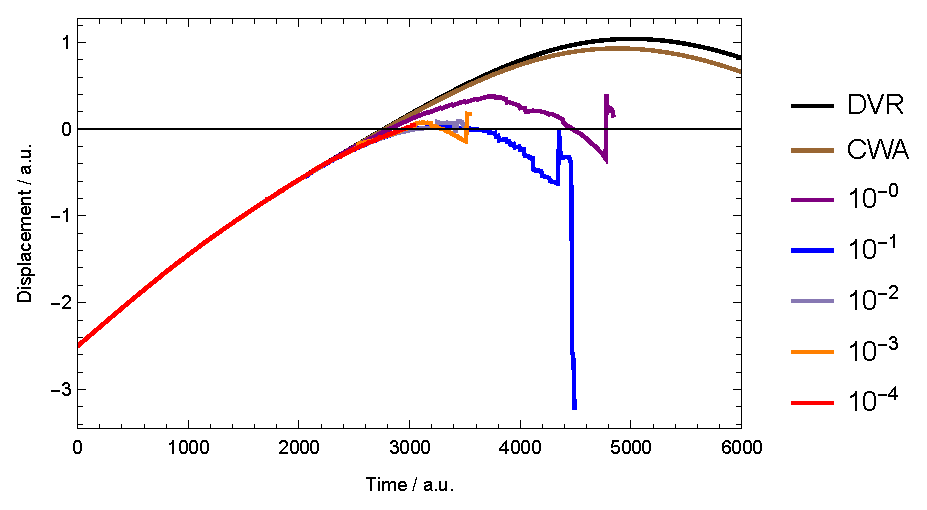
\includegraphics[width=0.48\textwidth]{SMD_CWA_OPT_init_7.eps}
}
\caption{不同的初始步长对SMD-CWA-OPT方法的影响}
\label{smd-cwa-opt-init}
\end{figure}

图 \ref{smd-cwa-opt-method}表现了不同的梯度收敛方式,其在每个维度使用50个格点共2500个格点,以0.01 a.u. 作为优化时的初始步长,$10^{-4} \, \mathrm{a.u.}$为惩罚函数收敛判定上限,$10^{-3}$为梯度收敛判定上限,每个演化时间步长为$10 \, \mathrm{a.u}$。从中可以看出,不同的收敛方法对体系有着一定的影响,对于高阶的影响显著强于对低阶的影响,这说明了高阶可观察量的期望值对于改变CWA分布的贡献。我们看到了相较于原先在$t = 4000 \, \mathrm{a.u.}$便偏离并数值崩坏的CWA-SMD方法,3阶SMD-CWA-OPT方法显现出良好的数值收敛性,即并没有发生数值崩坏。比较有意思的是对于5阶SMD-CWA-OPT方法中使用BFGS2方法时期望值变回到了精确解的附近,但由于GSL库报错而未能继续进行下去。因此后续的模拟皆采用了BFGS2作为梯度收敛方法。同时可以注意到,2阶在这里仍旧与CWA给出了相同的结果,这仍旧是由于二阶可观察量在磨雅括号里的演化方程形式与泊松括号下的演化方程相一致,因此SMD追踪的可观察量与CWA提供的物理量一直保持一致。

图 \ref{smd-cwa-opt-init}表现了不同的初始优化步长对体系的影响,其在每个维度使用50个格点共2500个格点,$10^{-4} \, \mathrm{a.u.}$为惩罚函数收敛判定上限,$10^{-3}$为梯度收敛判定上限,使用BFGS2方法,每个演化时间步长为$10 \, \mathrm{a.u}$。可以看出在发生分裂之前$10^{-2} \, \mathrm{a.u.}$便能够基本保持一定的收敛性,虽然比较有意思的是初始步长为$1 \, \mathrm{a.u.}$时其结果较接近于DVR或CWA方法,但由于收敛性问题我们不应该信任较大初始步长的结果——因为理论上初始步长越小越应收敛至惩罚函数的最小值,而我们设置的惩罚函数只有单一极值点。因此我们设定$10^{-2}$为初始步长。

同时我们能够看出在SMD-CWA-OPT仍旧出现了高阶的方法相对于低阶方法,模拟结果偏离精确解更快,波动幅度大,无法持续稳定运行等原因。值得注意的是,我们并没有完全地舍弃CWA分布在高阶可观察量的期望值——我们虽然试图通过利用较低阶的可观察量的期望值优化CWA的相空间分布,以使其更接近精确解提供的相空间分布,但其仍旧存在着高阶可观察量的期望值相对偏差较大的问题,而这些偏差仍旧会参与进SMD的演化方程中,而这些误差又反过来影响优化后的CWA分布。因此,虽然CWA方法与SMD方法能够形成一定程度上的``自洽'',提升了一定程度上的数值稳定性,但还远未达到能够提供更精确的模拟结果。

\subsection{CWA-SMD-OPT}
我们现针对由SMD追踪的位移、动量等可观察量的期望值来反映整个体系的的方法——SMD-CWA-OPT进行分析。由于CWA-SMD-OPT与SMD-CWA-OPT只相差期望值的提供的方式,而并未改变内部的任何实际数据,因此可以直接使用在SMD-CWA-OPT中探索出的一些优化条件。
\begin{figure}
\centering
\subfigure[3阶]{
  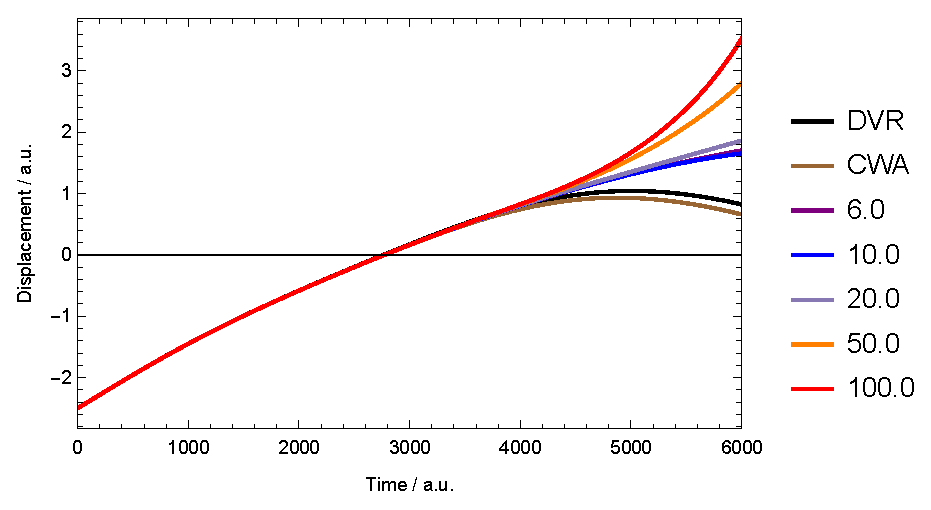
\includegraphics[width=0.48\textwidth]{CWA_SMD_OPT_dt_4.eps}
}
\subfigure[4阶]{
  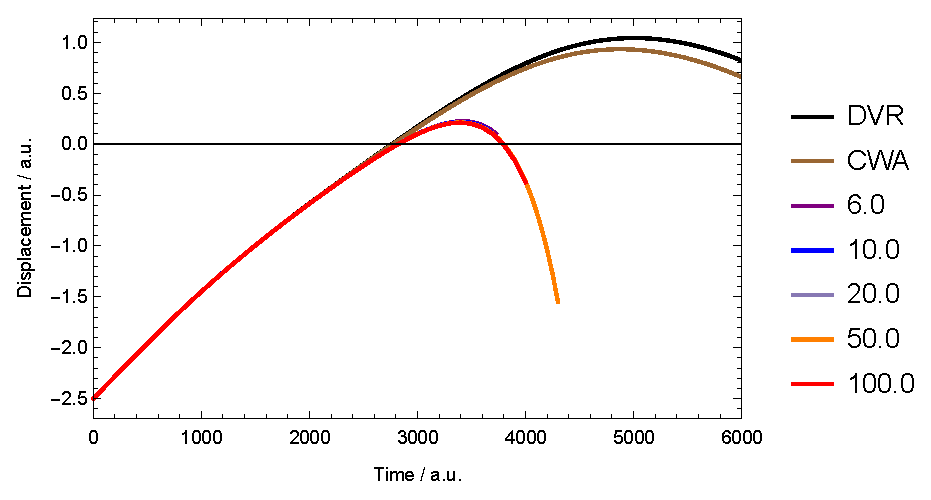
\includegraphics[width=0.48\textwidth]{CWA_SMD_OPT_dt_5.eps}
}
\subfigure[5阶]{
  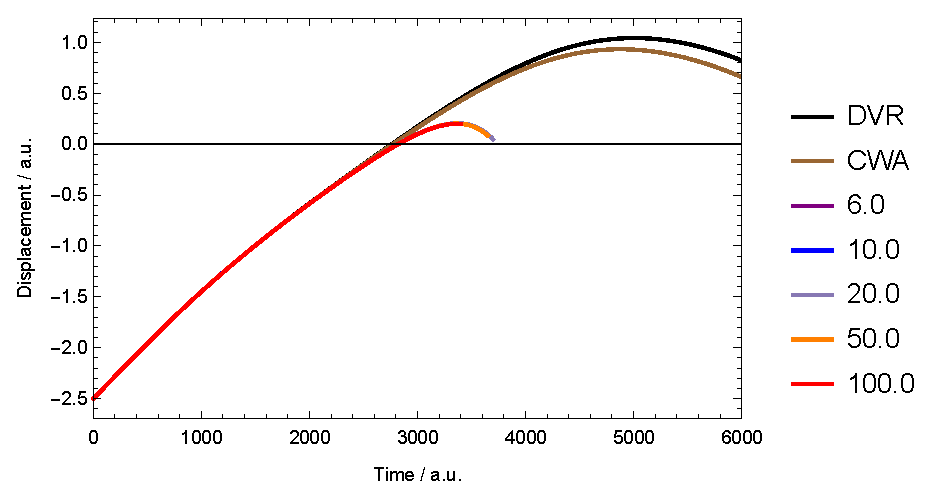
\includegraphics[width=0.48\textwidth]{CWA_SMD_OPT_dt_6.eps}
}
\subfigure[6阶]{
  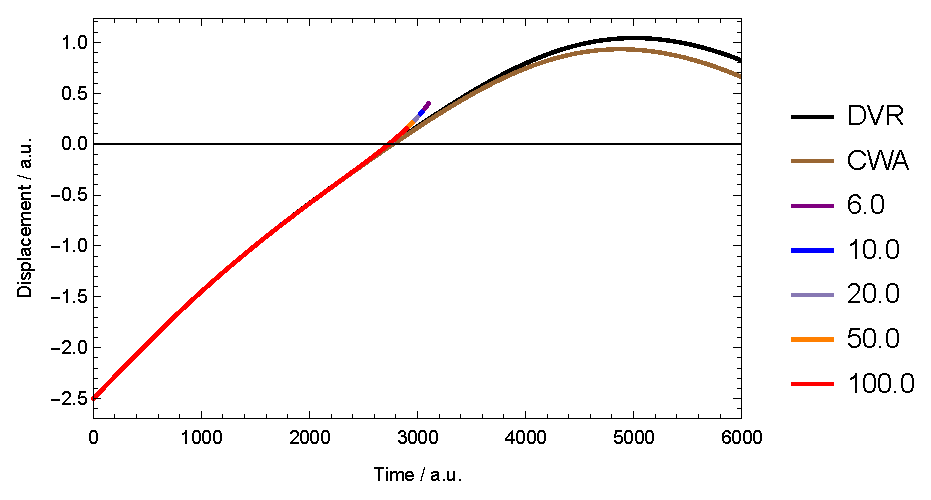
\includegraphics[width=0.48\textwidth]{CWA_SMD_OPT_dt_7.eps}
}
\caption{不同的初始步长对CWA-SMD-OPT方法的影响}
\label{cwa-smd-opt-dt}
\end{figure}

图 \ref{cwa-smd-opt-dt}表现了不同的时间步长对于模拟结果的影响。可以看出$t = 10 \, \mathrm{a.u.}$已基本处于收敛的状态。同时,相对于SMD-CWA-OPT方法,以SMD追踪的可观察量的期望值显现出了更强的数值稳定性,这一般是由于SMD自身的追踪的性质。但是我们仍旧看到了CWA-SMD的通病,即结果偏离精确解更快,波动幅度大,无法持续稳定运行等问题。

\begin{figure}
\centering
\subfigure[3阶]{
  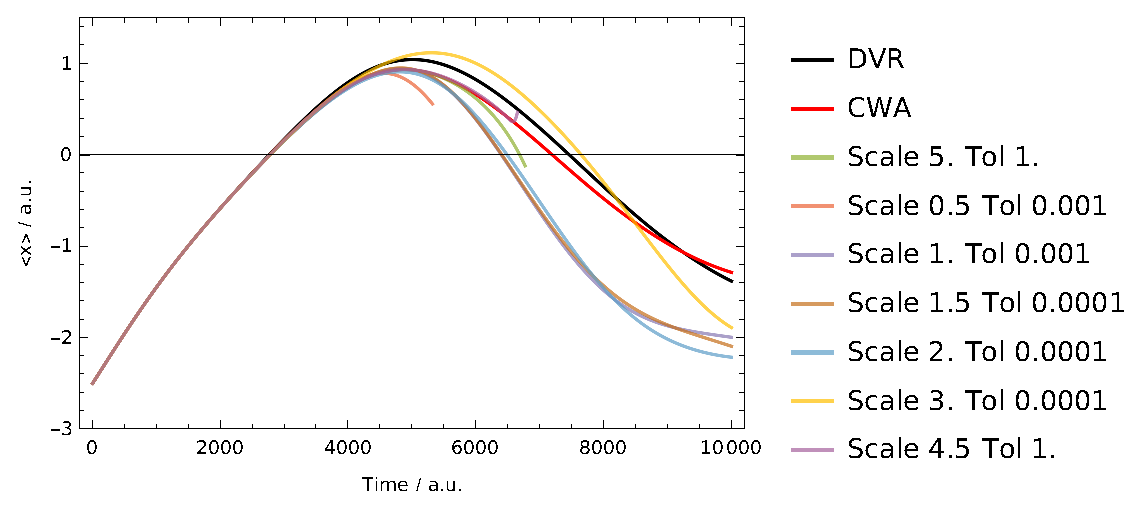
\includegraphics[width=1.0\textwidth]{Grade3_OPT.eps}
}
\subfigure[4阶]{
  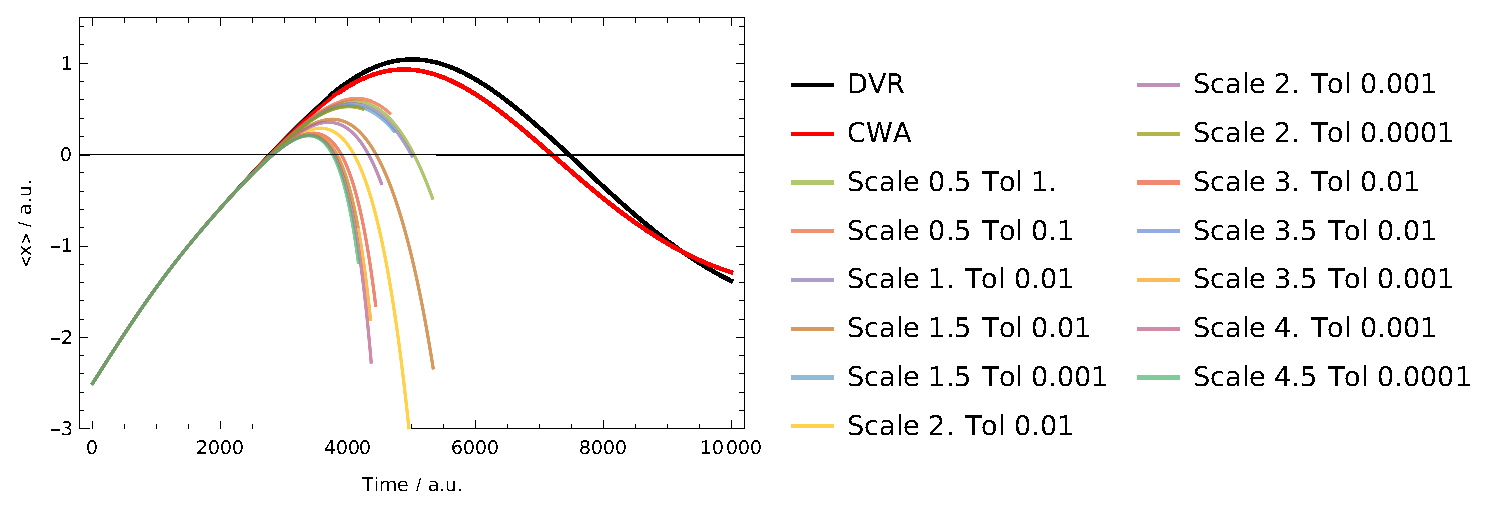
\includegraphics[width=1.0\textwidth]{Grade4_OPT.eps}
}
\subfigure[5阶]{
  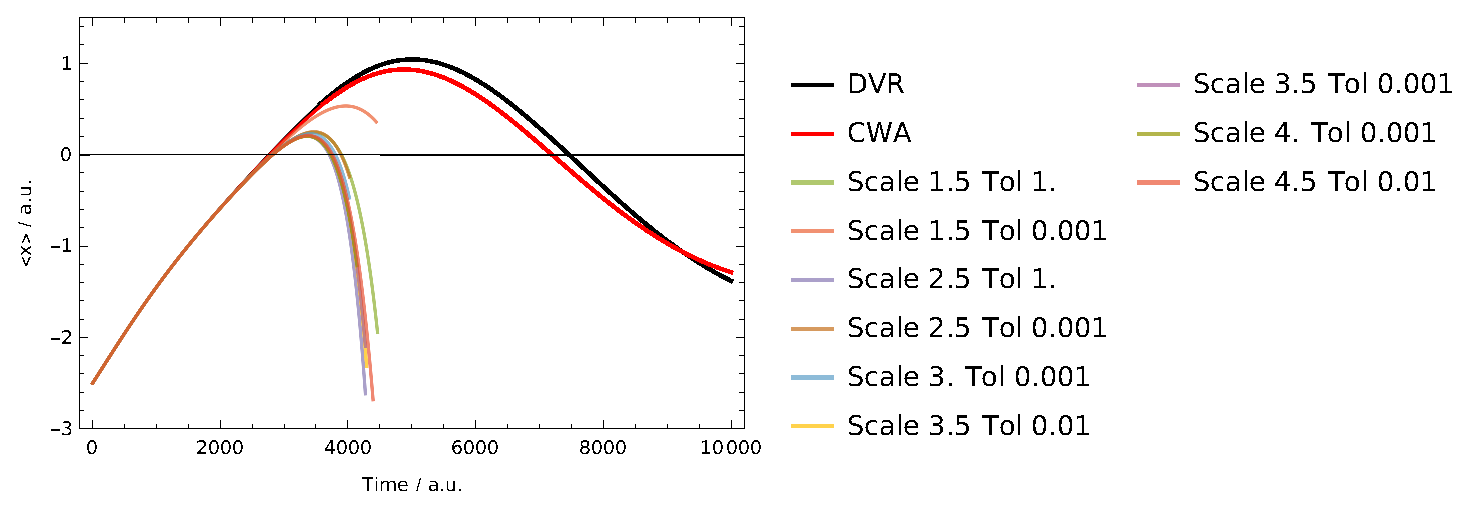
\includegraphics[width=1.0\textwidth]{Grade5_OPT.eps}
}
\caption{放缩系数以及收敛判定上限对CWA-SMD-OPT的影响}
\label{scaling-tolerance}
\end{figure}

由于放缩系数和收敛判定上限具有较大关联性——放缩系数的选择会极大地影响惩罚函数自身的数值,我们能对放缩系数和收敛判定进行了综合的测试,选择的放缩系数为$[0.5, 5.5]$每隔0.5取样,收敛判定上限为$10^{-k}, k \in [0,6] \cap \mathbb{N}$结果如图 \ref{scaling-tolerance}所示。